\documentclass[9pt]{beamer}
\usetheme[progressbar=frametitle]{metropolis}
\usepackage[ngerman]{babel}
\usepackage[utf8]{inputenc}
\usepackage{svg}
\usepackage{hyperref}
\usepackage{xtab}
\usepackage[T1]{fontenc}
\usepackage{lmodern}
\usepackage{caption}
\usepackage{algpseudocode}
\usepackage{booktabs} 
\usepackage{longtable}
\usepackage{amsmath}
\usepackage{booktabs}
\usepackage{multirow}
\usepackage{graphicx}
\usepackage{float}
\usepackage[dvipsnames]{xcolor}
\usepackage{amsfonts}
\usepackage{tikz}
\usetikzlibrary{shapes}
\usepackage{ marvosym }
%Theorems
\newtheorem{my}{Definition}
\title{Simultane Pfadzeichnungen auf dem Gitter}
\author{Timur Sultanov}
\date{Universität Trier, \today}

\begin{document}
    \maketitle
    \begin{frame}
    \frametitle{Motivation}
    \begin{itemize}
        \item \textbf{Simultaneous Embedding} = gleichzeitige Darstellung mehrerer Graphen mit gleicher Knotenmenge
        \item Besonders relevant bei nur geringfügigen Unterschieden\pause 
        \item \textbf{Ziel:} 
        \begin{itemize}
            \item Gemeinsame und differenzierende Strukturen visuell erfassbar machen
            \item Kompakte, konfliktfreie und gut lesbare Einbettung
        \end{itemize}
        \item \textbf{Herausforderungen:}
        \begin{itemize}
            \item Begrenzter Platz auf dem Gitter (Flächenminimierung)
            \item Minimierung der Biegungen zur Verbesserung der Lesbarkeit
            \item Vermeidung von Kreuzungen und Selbstüberschneidungen
        \end{itemize}
    \end{itemize}
\end{frame}

    \begin{frame}
    \frametitle{Ziel der Arbeit}
    \begin{itemize}
        \item Einbettung von zwei Pfaden auf einem Gitter
        \item Möglichst kompakt
        \item Pfade dürfen sich überlappen, aber nicht selbst schneiden
    \end{itemize} \pause

    \begin{figure}
        \centering
        \begin{minipage}{0.48\textwidth}
            \centering
            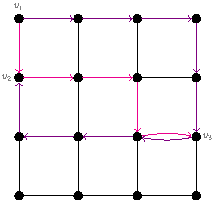
\includegraphics[width=\linewidth]{figures/Erlaubt.pdf}
            \caption*{\textbf{(a)} Erlaubte Zeichnung}
        \end{minipage}\hfill
        \begin{minipage}{0.48\textwidth}
            \centering
            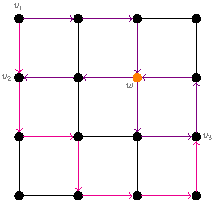
\includegraphics[width=\linewidth]{figures/Unerlaubt.pdf}
            \caption*{\textbf{(b)} Verbotene Zeichnung}
        \end{minipage}
    \end{figure}
\end{frame}

\begin{frame}{Ziel der Arbeit}
    Möglichst kompakt/Flächenminimierend
    \begin{figure}
        \centering
        \begin{minipage}{0.48\textwidth}
            \centering
            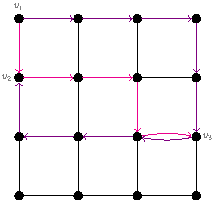
\includegraphics[width=\linewidth]{figures/Erlaubt.pdf}
        \end{minipage}\hfill
        \begin{minipage}{0.48\textwidth}
            \centering
            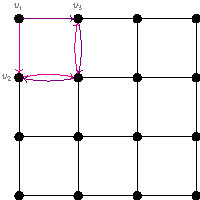
\includegraphics[width=\linewidth]{figures/Erlaubt2.pdf}
        \end{minipage}
    \end{figure}
\end{frame}

    \begin{frame}
    \frametitle{Lineare \& ganzzahlige Optimierung}
    \textbf{Lineare Optimierung(LP):} Optimierung einer linearen Zielfunktion unter linearen Nebenbedingungen \newline
    \textbf{Ganzzahlige lineare Programmierung (ILP):} Variablen dürfen \textbf{nur ganzzahlige Werte }annehmen
    \vspace{0.5em}
    \pause \newline
    \begin{columns}
    \begin{column}{0.5\textwidth}
        
    \textbf{Beispiele für ILP-Anwendungen:}
    
    \begin{itemize}
        \item Travelling Salesman Problem
        \item quadratische Zuordnungsproblem
        \item Knapsack Problem
    \end{itemize}
    \end{column}
    \begin{column}{0.3\textwidth}
    \centering
    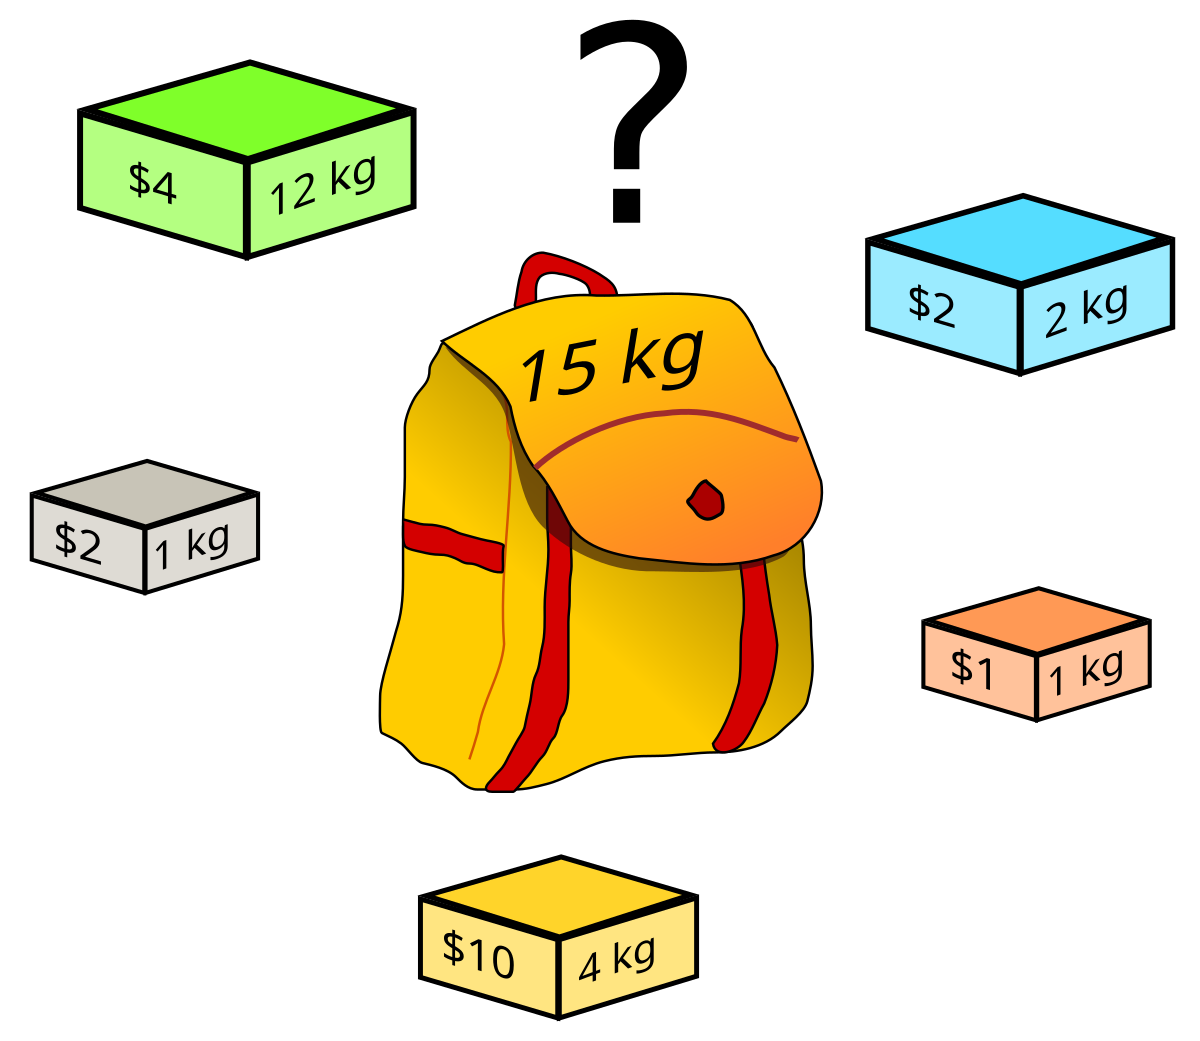
\includegraphics[width=\textwidth]{figures/Knapsack.png}
  \end{column}
\end{columns}
    \end{frame}

    \begin{frame}
    \frametitle{Implementierung in Python mit gurobipy}
    \begin{itemize}
        \item Große Lesbarkeit und Wartbarkeit des Codes
        \item Nahtlose Einbettung von Gurobi via gurobipy API
        \item Obwohl Python langsamer als C++ ist, hat das keine negativen Auswirkungen, da die eigentliche Lösung im Gurobi-Core (C++) abläuft
    \end{itemize}\pause 
    Gurobi als leistungsstarker ILP-Solver:
    \begin{itemize}
        \item Kein eigener Algorithmus notwendig
        \item nutzt \textit{hybride Verfahren} zur Lösung von ILPs
    \end{itemize}\pause 
    In einer Vergleichstudie(2023) wurden fünf kommerzielle und freie ILP-Solver gegenübergestellt: Gurobi zählt zu den \textbf{schnellsten und zuverlässigsten} Solvern
    
    \end{frame}
    
    \begin{frame}
    \frametitle{Variablen des ILP-Modells}
    \begin{columns}
  \begin{column}{0.45\textwidth}
    \textbf{Zuweisung von Knoten zu Gitterpunkten:}
    \[
    \sigma(v, p) =
    \begin{cases}
    1, & \text{falls } v \text{ auf Gitterpunkt } p \text{ liegt} \\
    0, & \text{sonst}
    \end{cases}
    \]

    \vspace{0.5em}
    \textbf{Belegung von Gitterkanten durch Pfadkanten:}
    \[
    \mu(e, p, q) =
    \begin{cases}
    1, & \text{falls } e \text{ die Gitterkante } (p, q) \text{ nutzt} \\
    0, & \text{sonst}
    \end{cases}
    \]
  \end{column}
  \pause 
  \begin{column}{0.4\textwidth}
    \centering
    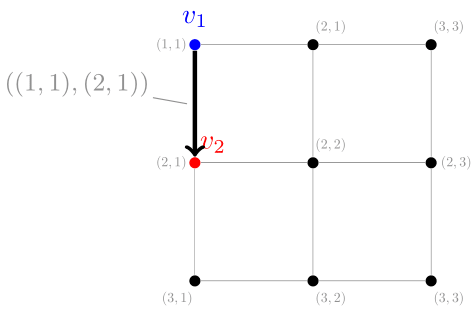
\includegraphics[width=\textwidth]{figures/Variabelsetzung.pdf}
  \end{column}
\end{columns}\pause 
\vspace{0.5em}
\textbf{Zielfunktion:} $Z = \sum_{e \in E} \sum_{(p,q) \in F} \mu(e,p,q)$
    \end{frame}

    \begin{frame}
    \frametitle{Nebenbedingungen}
    \begin{enumerate}[(1)]
    \item  Jeder Knoten muss auf genau einem Gitterpunkt liegen
    \item Auf einem Gitterpunkt darf höchstens ein Knoten liegen \pause 
    \item Kanten müssen kontinuierlich gezeichnet werden
    \item Kanten dürfen keine Gitterpunkte durchlaufen, an dem ein Knoten liegt, der nicht zu der jeweiligen Kante inzident ist
    \item Es darf keine Überschneidungen innerhalb eines Pfades geben
    \end{enumerate}
    \end{frame}

    \begin{frame}{Nebenbedingungen}
    (1) Jeder Knoten muss auf genau einem Gitterpunkt liegen:
        $$\forall v \in V \sum_{p \in P} \sigma(v,p) = 1$$
            (2) Auf einem Gitterpunkt darf höchstens ein Knoten liegen:
            $$\forall p \in P \sum_{v \in V} \sigma(v,p) \leq 1$$
    \end{frame}

    \begin{frame}{Nebenbedingungen}
    (3) Kanten müssen kontinuierlich gezeichnet werden:
    \begin{figure}[H]
    \begin{minipage}{0.35\textwidth}
    \centering
    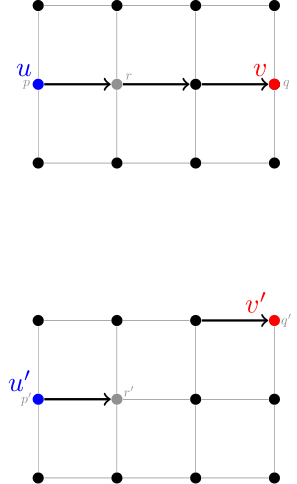
\includegraphics{figures/Kontinuierlich.pdf}
    \label{fig:Kontinuierlich}
    \end{minipage}
    \begin{minipage}{0.57\textwidth}
    \pause 
    $$\forall e=(u,v) \in E, u,v \in V, \forall p \in D:$$ $$\sum_{(p,q) \in F} \mu(e,p,q) - \sum_{(q,p) \in F} \mu(e,q,p) = \sigma(u,p) - \sigma(v,p)$$
    \end{minipage}
\end{figure}
    \end{frame}

    \begin{frame}{Nebenbedingungen}
        (4) Kanten dürfen keine Gitterpunkte durchlaufen, an dem ein Knoten liegt, der nicht zu der jeweiligen Kante inzident ist:
        \newline 
        Summe aller eingehenden und ausgehenden genutzten Gitterkanten am Gitterpunkt $p$ von einer Kante $e$: $$flow\_sum = \sum_{(p,q) \in F} \mu(e,p,q) + \sum_{(q,p) \in F} \mu(e,q,p)$$\pause 
        \begin{figure}[H]
            \centering
            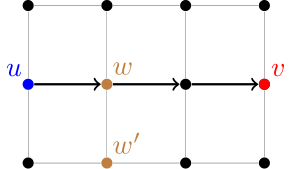
\includegraphics{figures/OverNodePoint.pdf}
            \label{fig:OverNodePoint}
        \end{figure}
        $$flow\_sum \leq 2 \cdot (1 - \sigma(w,p))$$
    \end{frame}

    \begin{frame}{Nebenbedingungen}
        (5) Es darf keine Überschneidungen innerhalb eines Pfades geben: \newline \par 
        Sei nun $W$ die Menge an Pfaden. Für alle $P_i =(V_i, E_i) \in W$ und für jeden Gitterpunkt $p \in D$ definieren wir die aggregierte Anzahl an korrespondierenden Gitterkanten an $p$, die von den Kanten $e_i \in E_i$ genutzt werden: $$aggregated\_flow = \sum_{e \in p_i}(\sum_{(p,q) \in F} \mu(e,p,q) + \sum_{(q,p) \in F} \mu(e,q,p))$$ \pause
        Nun gibt es zwei Szenarien für jeden Pfad:
        \begin{itemize}
            \item Gitterpunkt $p$ wird nicht passiert $\rightarrow aggregated\_flow = 0$
            \item Gitterpunkt $p$ wird passiert $\rightarrow aggregated\_flow = 1 \lor 2$
        \end{itemize}
        $$aggregated\_flow \leq 2$$
    \end{frame}

    \begin{frame}
    \frametitle{Testinstanzen und Gitterwahl}
    \textbf{1. Testreihe:}
    \begin{itemize}
        \item 10 zufällige Testfälle für $5-11$ Knoten
        \item Wahl des Gitters: $(\left\lceil n/2 \right\rceil+1 \times \left\lceil n/2 
        \right\rceil+1)$\pause 
        \end{itemize}
        \textbf{2. Testreihe:}
        \begin{itemize}
        \item Anzahl gleicher adjazenter Knoten für Pfade mit 10 Knoten
        \item jeweils 10 Testfälle
    \end{itemize}
    \end{frame}

    \begin{frame}
    \frametitle{Modellkomplexität}
    \begin{figure}
        \centering
        \begin{minipage}{0.48\textwidth}
            \centering
            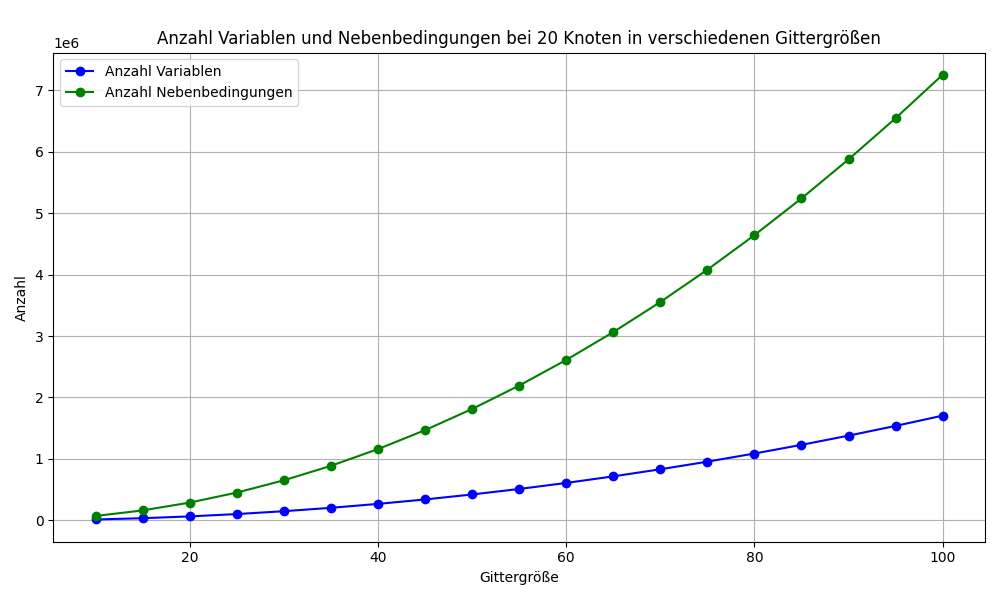
\includegraphics[width=\linewidth]{figures/20NodesVarNEb.png}
        \end{minipage}\hfill
        \begin{minipage}{0.48\textwidth}
            \centering
            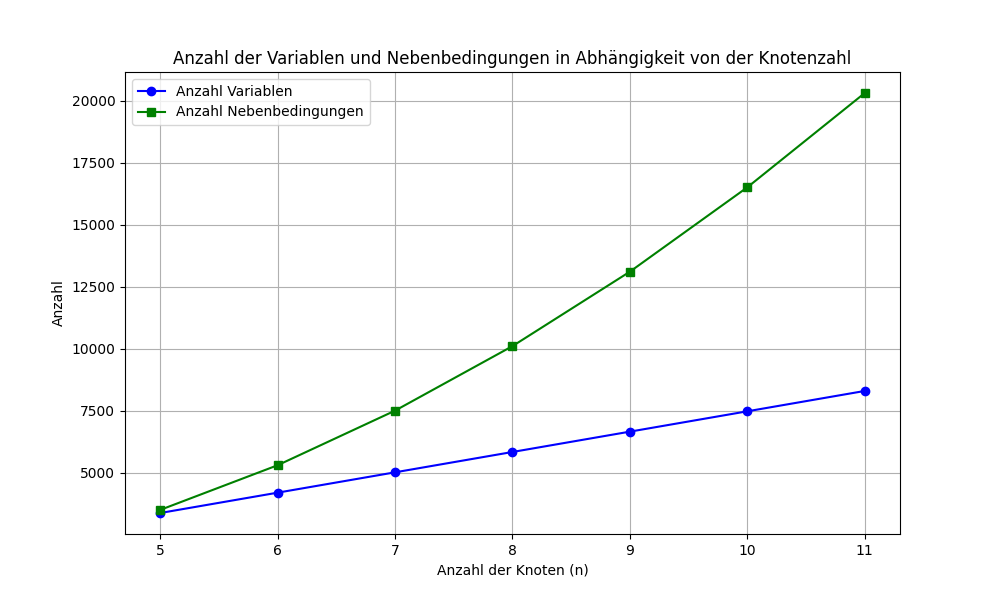
\includegraphics[width=\linewidth]{figures/VariabelConstrains5-11.png}
        \end{minipage}
    \end{figure}
    \end{frame}

    \begin{frame}
    \frametitle{Laufzeiten bei fester Knotenzahl: $5\times5$ vs. $8\times8$ Gitter}
    \begin{figure}
        \centering
        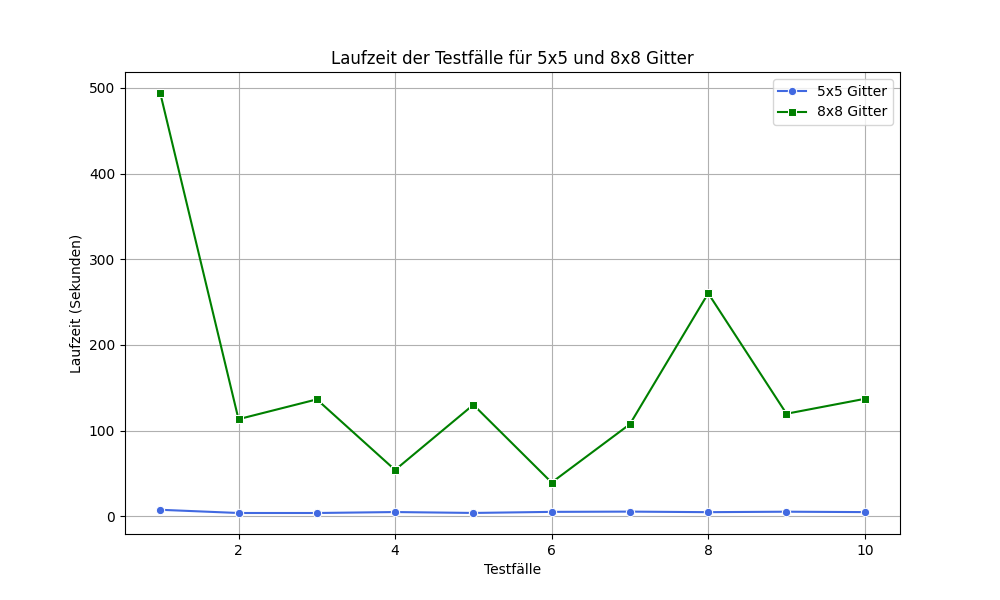
\includegraphics[width=\textwidth]{figures/Laufzeit8NodesDiffOneY.png}
    \end{figure}
    \end{frame}

    \begin{frame}
    \frametitle{Laufzeiten bei wachsender Knotenzahl (5–11)}
    \begin{figure}
        \centering
        \begin{minipage}{0.48\textwidth}
            \centering
            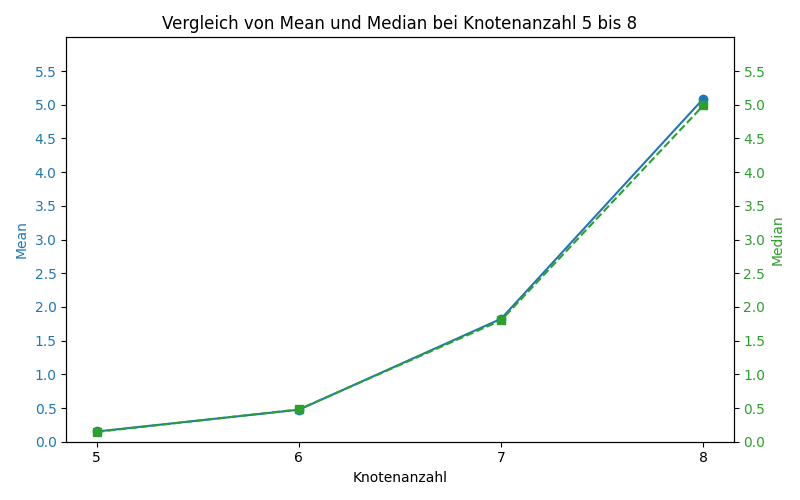
\includegraphics[width=\linewidth]{figures/Mean_Medain5-8.png}
        \end{minipage}\hfill
        \begin{minipage}{0.48\textwidth}
            \centering
            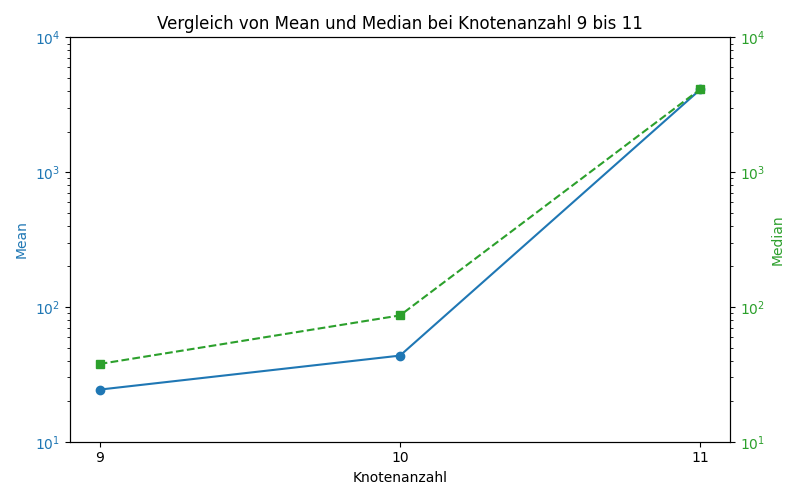
\includegraphics[width=\linewidth]{figures/Mean_Medain9-11.png}
        \end{minipage}
    \end{figure}
    \end{frame}

    \begin{frame}
    \frametitle{Ursachen für Laufzeitschwankungen bei 10 Knoten}
    \textit{Mögliche Ursachen:}
    \begin{itemize}
        \item Wert der Zielfunktion
        \item Anzahl gleicher adjazenter Knoten
        \item Komplexität der resultierenden Einbettung
    \end{itemize}
    \end{frame}

    \begin{frame}{Ursachen für Laufzeitschwankungen bei 10 Knoten}
        \begin{figure}
        \centering
        \begin{minipage}{0.48\textwidth}
            \centering
            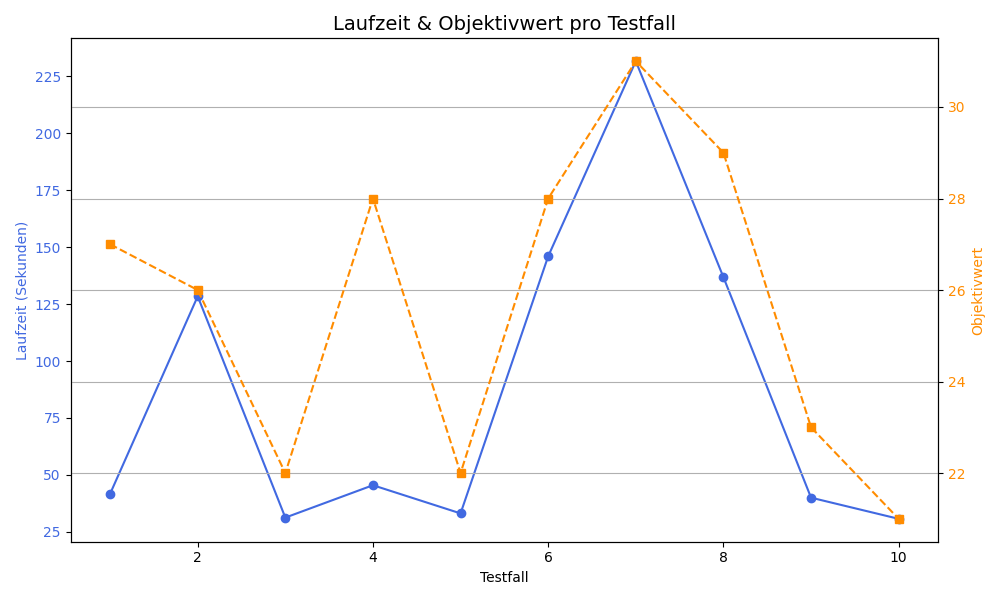
\includegraphics[width=\linewidth]{figures/LaufzeitObjektivwert10.png}
        \end{minipage}\hfill
        \begin{minipage}{0.48\textwidth}
            \centering
            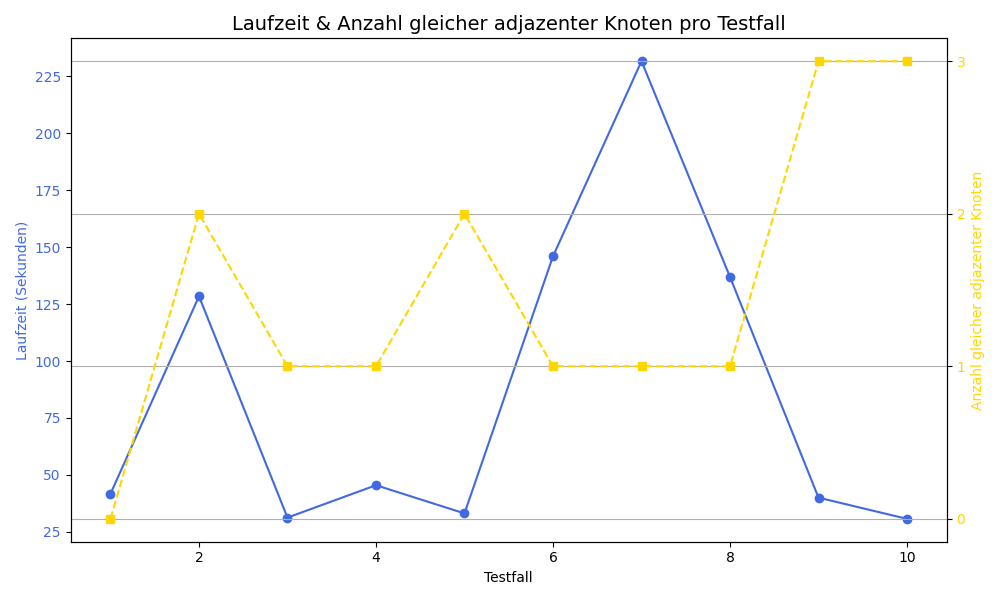
\includegraphics[width=\linewidth]{figures/LaufzeitAdjNodes10.png}
        \end{minipage}
    \end{figure}
    \end{frame}

\begin{frame}
    \frametitle{Graphische Darstellung der Testfälle}

    \begin{minipage}{0.48\textwidth}
        \centering
        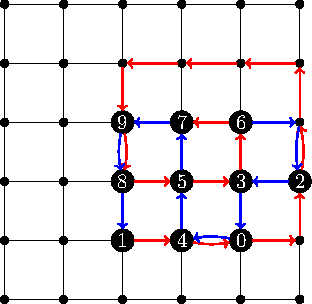
\includegraphics[height=3.2cm]{figures/Testfall3.pdf}
        \captionof*{figure}{Testfall 3: 31,22s}
    \end{minipage}
    \hfill
    \begin{minipage}{0.48\textwidth}
        \centering
        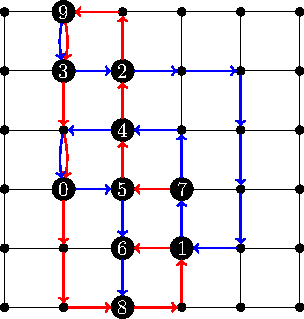
\includegraphics[height=3.2cm]{figures/Testfall4.pdf}
        \captionof*{figure}{Testfall 4: 45,44s}
    \end{minipage}

    \vspace{0.3cm}

    \begin{minipage}{0.48\textwidth}
        \centering
        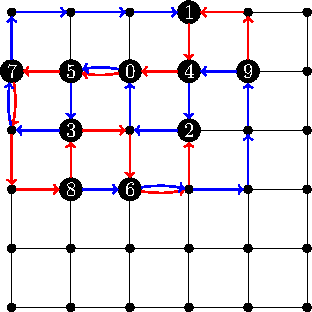
\includegraphics[height=3.2cm]{figures/Testfall6.pdf}
        \captionof*{figure}{Testfall 6: 145,99s}
    \end{minipage}
    \hfill
    \begin{minipage}{0.48\textwidth}
        \centering
        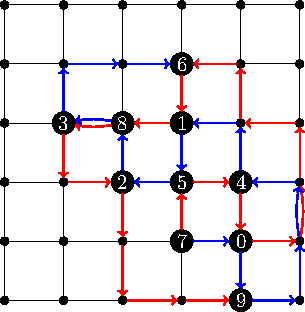
\includegraphics[height=3.2cm]{figures/Testfall7.pdf}
        \captionof*{figure}{Testfall 7: 231,68s}
    \end{minipage}

\end{frame}

\begin{frame}
    \frametitle{Laufzeiten und Pfadlängenverteilung bei 10 Knoten}

    \begin{columns}
        % Linke Spalte – Tabelle
        \begin{column}{0.55\textwidth}
            \scriptsize
            \begin{tabular}{|c|c|c|}
                \hline
                \textbf{Testfall} & \textbf{Laufzeit (s)} & \textbf{Kanten (L:A)} \\
                \hline
                1 & 41{,}64 & 2:4, 3:1, 6:1 \\
                2 & 128{,}42 & 2:4, 3:1, 7:1 \\
                3 & 31{,}22 & 2:2, 6:1 \\
                4 & 45{,}44 & 2:5, 3:1, 6:1 \\
                5 & 33{,}06 & 2:3, 5:1 \\
                6 & 146{,}00 & 2:5, 3:2, 4:2 \\
                7 & 231{,}68 & 2:2, 3:1, 4:2, 6:1 \\
                8 & 136{,}91 & 2:2, 3:1, 4:3 \\
                9 & 39{,}98 & 2:4, 3:2 \\
                10 & 30{,}67 & 2:3, 3:2 \\
                \hline
            \end{tabular}
        \end{column}

        % Rechte Spalte – Erklärender Text
        \begin{column}{0.4\textwidth}
            \footnotesize
            \textbf{Beobachtungen:}
            \begin{itemize}
                \item Höhere Laufzeiten bei komplexerer Struktur
                \item Viele Kanten mit Länge > 1 erhöhen die Rechenzeit
                \item Kürzere, kompakte Pfade führen zu schnelleren Lösungen
            \end{itemize}
        \end{column}
    \end{columns}
\end{frame}


    \begin{frame}
    \frametitle{Laufzeitverhalten bei steigender Anzahl identischer adjazenter Knoten}
    \begin{figure}
        \centering
        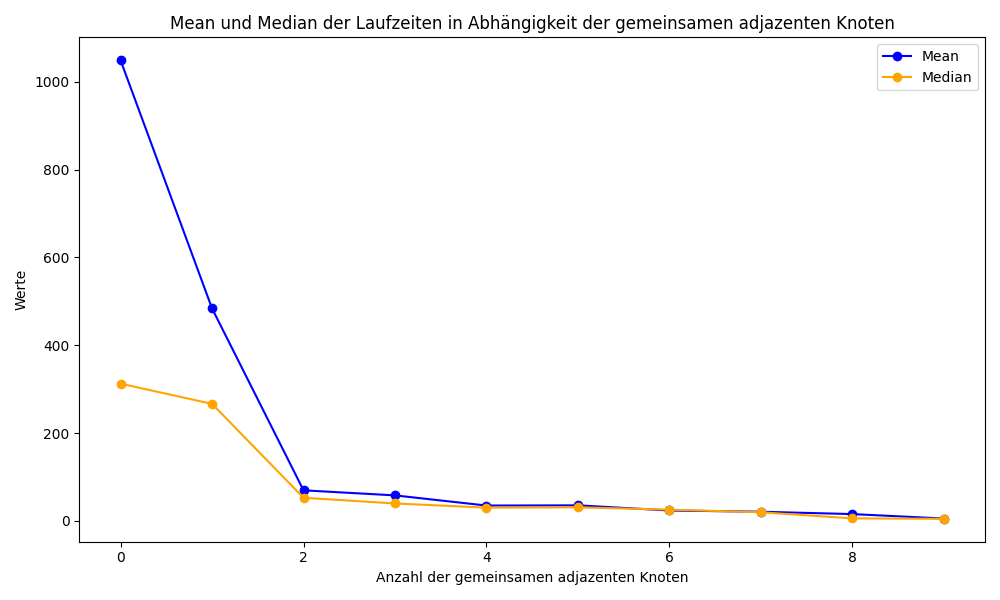
\includegraphics[width=\textwidth]{figures/SimMeanMedian.png}
    \end{figure}
    \end{frame}

    \begin{frame}
    \frametitle{Fazit: Bewertung des Modells}
    \begin{itemize}
        \item Für kleine Instanzen ($\leq$ 8 Knoten) sehr zuverlässig und schnell
        \item Rechenzeiten stabil und gut prognostizierbar
        \item Ab 12 Knoten: drastischer Anstieg der Laufzeit (bis Stunden/Tage)
        \item Gründe:
        \begin{itemize}
            \item Große Gitter $\Rightarrow$ viele Variablen \& Nebenbedingungen
            \item Komplexere Pfade mit Überlappungen und langen Kanten
        \end{itemize}
        \item Modell ist konzeptionell korrekt, aber skaliert nicht gut
    \end{itemize}
    \end{frame}

    \begin{frame}
    \frametitle{Optimierungsmöglichkeiten}
    \textbf{Ziel: Verbesserung der Skalierbarkeit und Laufzeit}
    \begin{itemize}
        \item \textbf{Heuristische Verfahren:}
        \begin{itemize}
            \item Greedy, Simulated Annealing, etc.
            \item Schnell gute Lösungen für große Instanzen
            \item Können als obere Schranke dienen
        \end{itemize}
        \item \textbf{Vorverarbeitung der Eingabe:}
        \begin{itemize}
            \item Graphvereinfachung, Symmetrieerkennung
            \item Reduktion unnötiger Redundanz im Modell
        \end{itemize}
    \end{itemize}
\end{frame}


\end{document}